% Author: Filip Bartek

Slinky is a spring-like toy invented by a naval engineer Richard James
between the years 1943 and 1945.\cite{bellis:historyofslinky}
It quickly became popular in the United States and it is still
widely available nowadays (see figure \ref{fig:slinky-original}).
Various unofficial Slinky duplicates can be found in shops
around Slovenia and Czech Republic and various e-shops
(see an example in figure \ref{fig:slinky-magic}).

\begin{figure}
  \centering
  %\includegraphics[height=7cm]{100-Slinky-Image.jpg}
  \includegraphics[width=\linewidth]{100-Slinky-Image.jpg}
  % Source:
  % http://poof-slinky.com/product/3pk-original-metal-slinky/?pcat_id=301
  \caption{Original Metal Slinky (2014)\cite{poof:slinky}}
  \label{fig:slinky-original}
\end{figure}

\begin{figure}
  \centering
  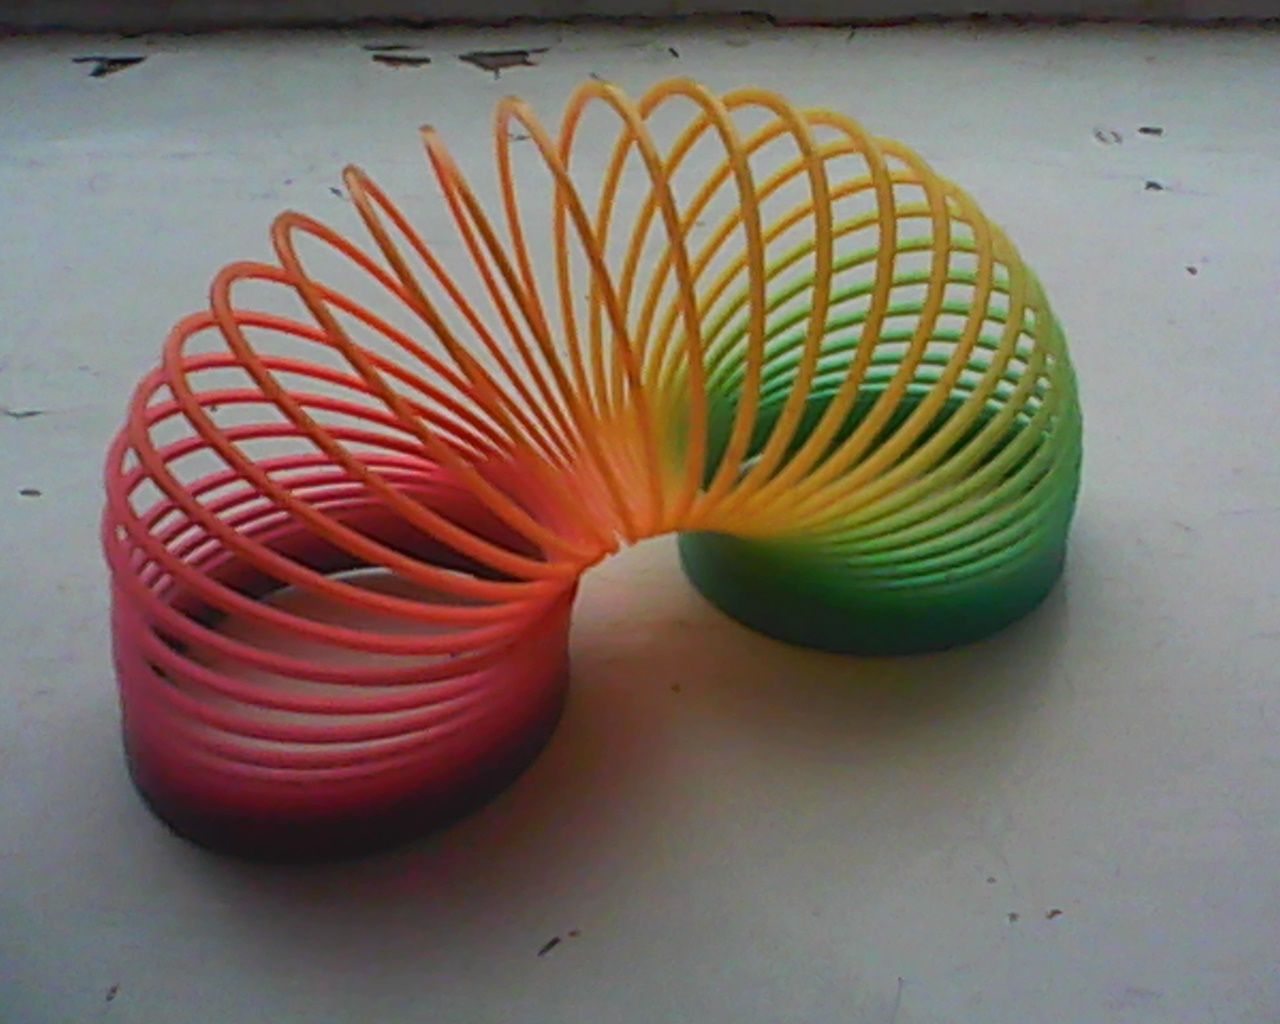
\includegraphics[width=\linewidth]{slinky-magic.jpg}
  \caption{Magic Spring, an unofficial duplicate of the plastic Slinky}
  \label{fig:slinky-magic}
\end{figure}

The physical properties of the toy make it suitable for juggling.
The original manufacturer exposed this potential in
a 1960s TV commercial\cite{youtube:slinky_commercial}
but the overall cultural influence of Slinky juggling
has been extremely limited.

A notable exception
and at the same time a good example of basic Slinky juggling,
which will be referred to as ``slinky walking'' from now on,
can be seen in a video from the \emph{YouTube} user
\emph{tyranicslinky}.\cite{youtube:tyranicslinky}.

\slinkyconductor{} is an imagined software music toy that
plays back music synchronized to a Slinky juggler's performance.

This text describes the development and functionality of
a prototype of \slinkyconductor{}.

In the remainder of the text, we will use the term \emph{slinky}
(with lowercase \emph{s}) as a common name for both
the original Slinky toys and
the unofficial duplicates.
We decided to do so because from the point of view of both
a slinky juggler and
a \slinkyconductor{} user
there is virtually no difference between the two variants of the toy.
However, there \emph{is} significant difference between
metal and plastic slinkys
(see figures \ref{fig:slinky-original} and \ref{fig:slinky-magic}
respectively),
which we will deal with in the next section.
